\subsubsection{\textit{World service}}

El \textit{world service} es el encargado de gestionar los mundos y sus zonas, así como la orquestación de los
servidores de juego asociados a cada una de ellas. El servicio se divide en tres componentes principales: la
gestión de mundos, la gestión de zonas y el registro de servidores.
\vspace{0.25cm}

Un mundo se crea mediante \texttt{POST /world}, donde el usuario proporciona un nombre, una descripción y los
datos de configuración del mundo en formato JSON. El nombre debe tener entre 1 y 24 caracteres, sin espacios ni
caracteres especiales, y debe ser único en el sistema; de lo contrario, se retorna un error de conflicto. Esto proporciona
un ID al mundo en los datos del mundo (\textit{world data}), con el cual se puede actualizar el mundo ya creado con
\texttt{PUT /world/\{id\}}. Adicionalmente, mundo almacena además un campo \texttt{createable\_data}, que contiene la 
configuración de los objetos que pueden ser instanciados en él y que puede actualizarse de forma independiente mediante
\texttt{PUT /world/\{id\}/createable-data}.
\vspace{0.25cm}

La consulta de un mundo se realiza mediante \texttt{GET /world/\{id\}}, que retorna la configuración completa
junto con los metadatos de sus zonas. El listado de mundos se obtiene mediante \texttt{GET /world}, que admite
paginación a través de los parámetros obligatorios \texttt{offset} y \texttt{limit}, con un máximo de 100
resultados por página, y permite filtrar por propietario mediante el parámetro opcional \texttt{user\_id}. 
\vspace{0.25cm}

Cada mundo se divide en zonas, identificadas por un número entero positivo. Una zona se publica o actualiza
mediante \texttt{PUT /world/\{id\}/zones/\{zone\_id\}}, operación que requiere que el usuario sea propietario
del mundo. Cada zona almacena sus propios datos de configuración en formato JSON y expone dos indicadores de
estado: \texttt{is\_active}, que indica si la zona tiene un servidor de juego asignado, e \texttt{is\_online},
que indica si dicho servidor está en ejecución en ese momento.
\vspace{0.25cm}

\begin{figure}[h]
    \centering
    \begin{adjustbox}{width=1.10\textwidth, center}
        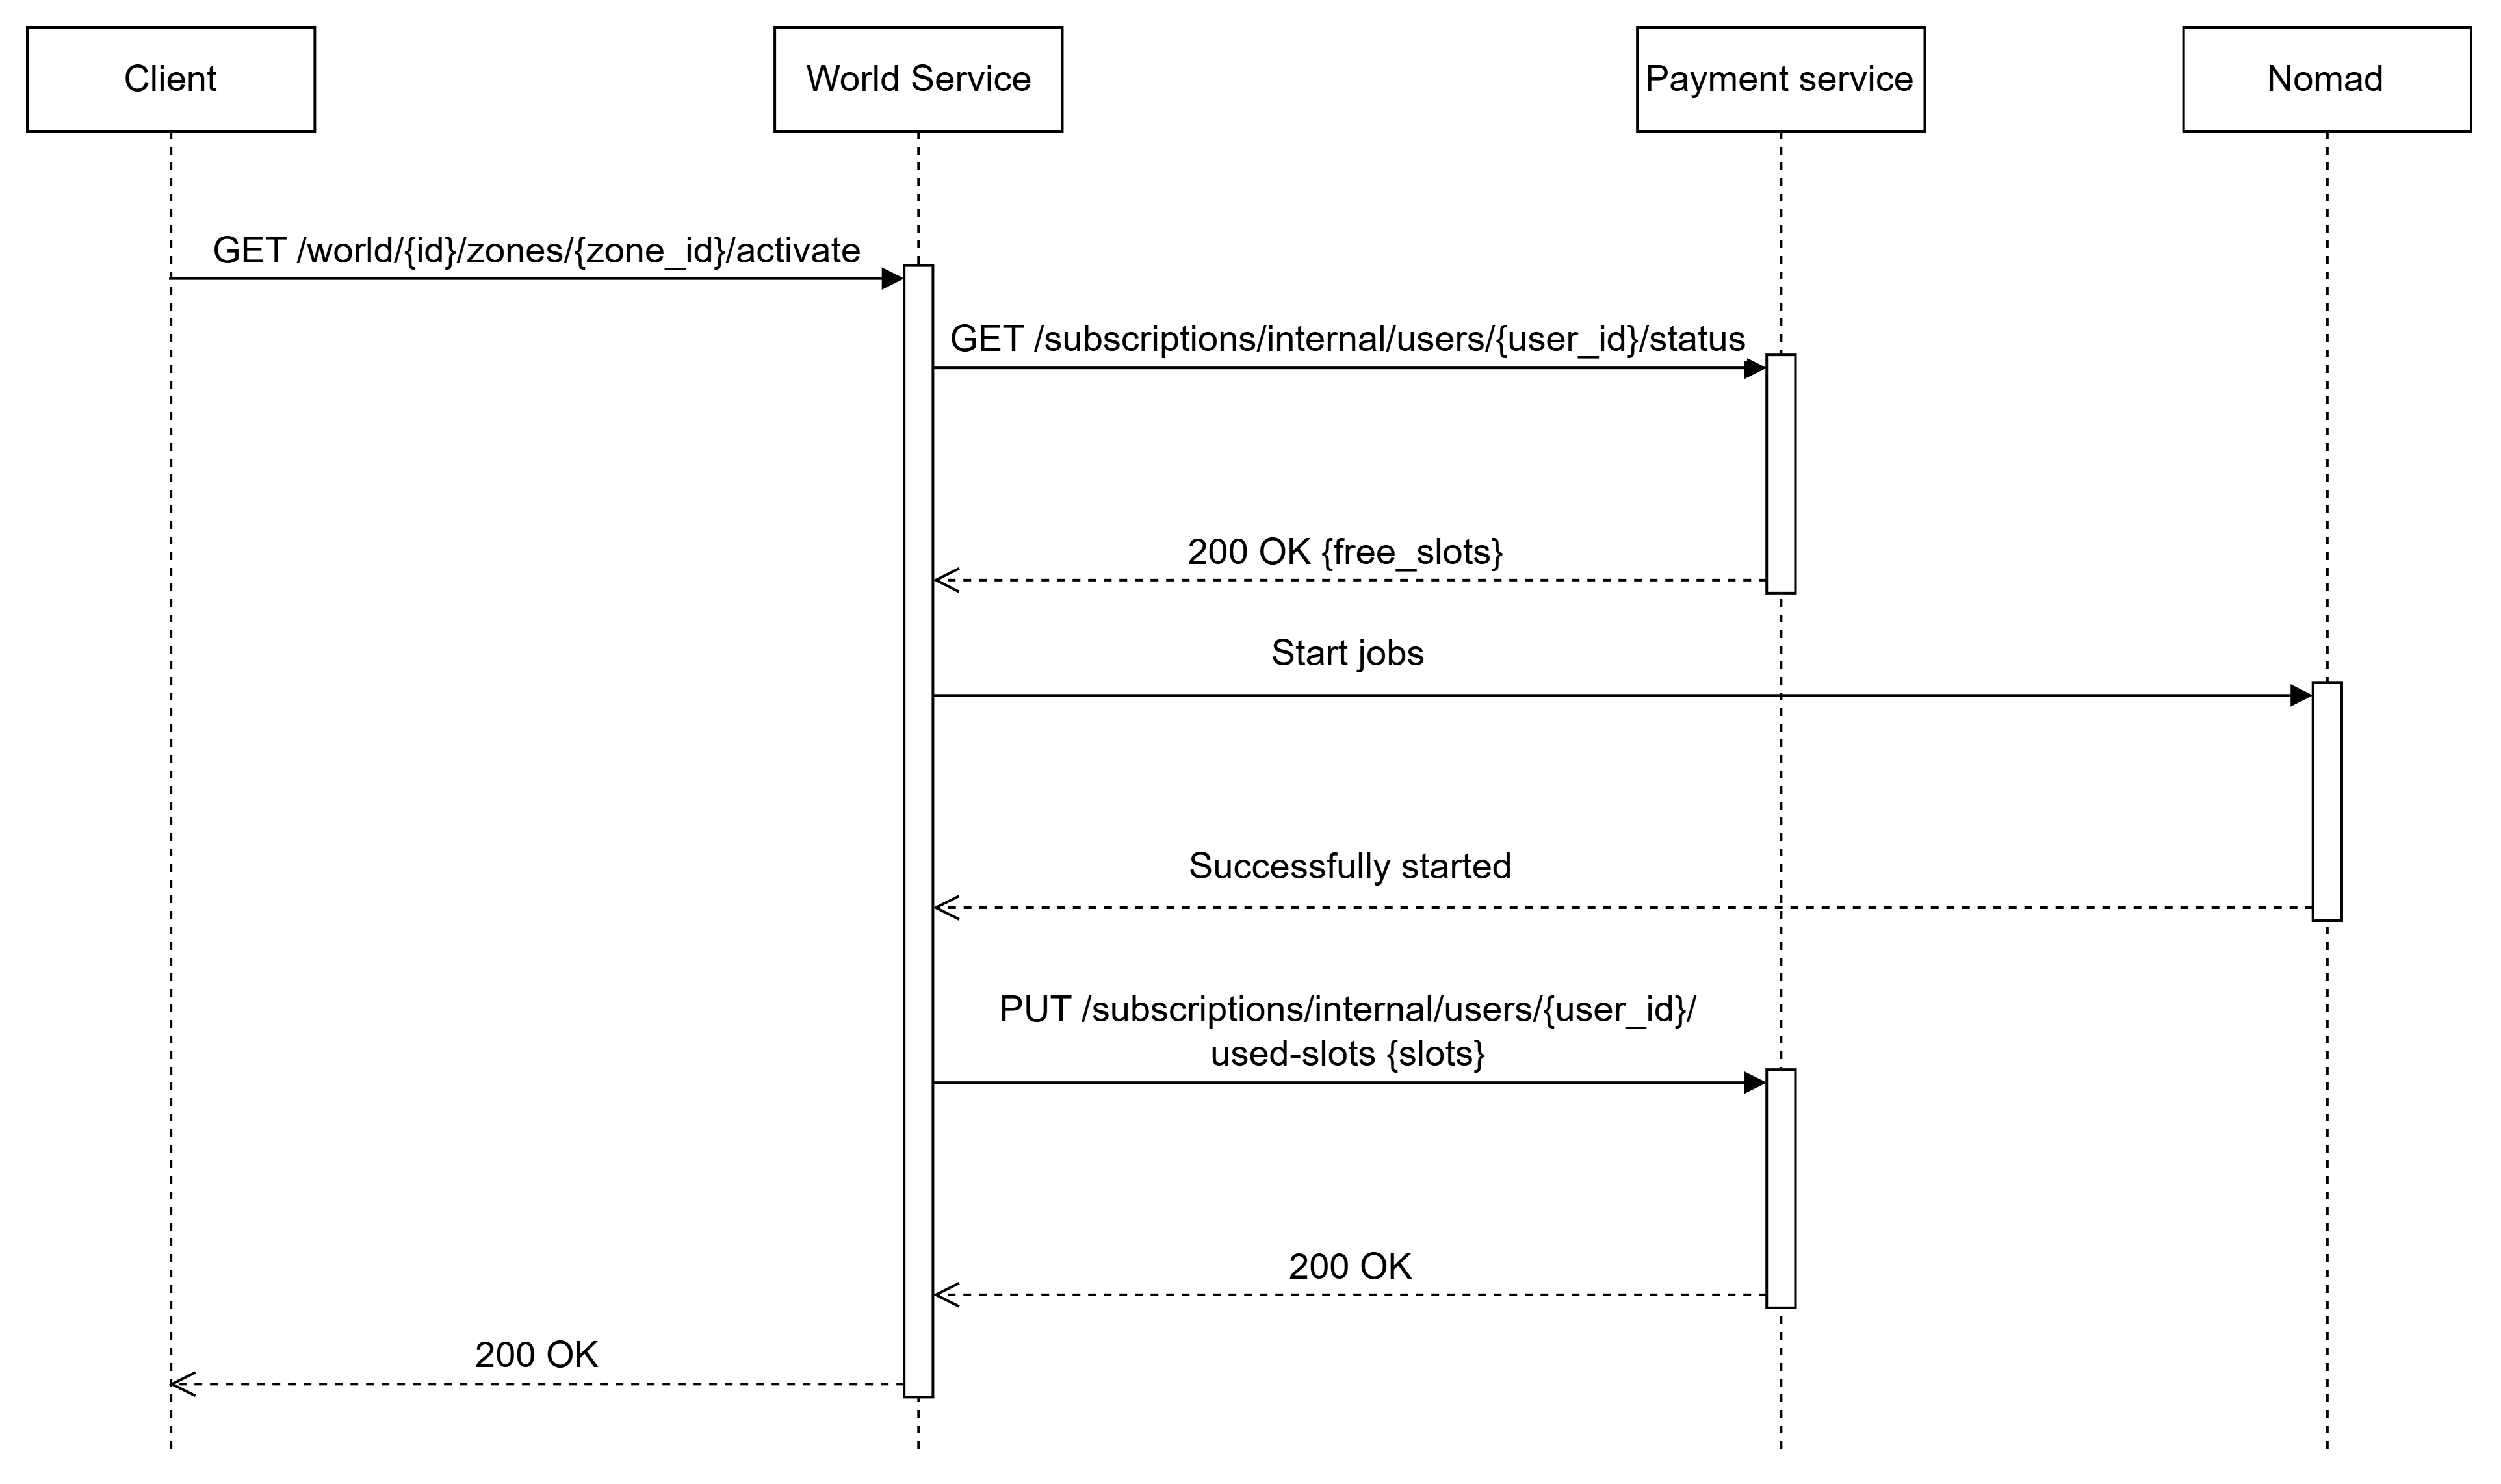
\includegraphics{img/08-implemented-solution/core-service/world-service-case-1.png}
    \end{adjustbox}
    \caption{Diagrama de secuencia del consumo de un \textit{slot}}
    \label{fig:world-service-case-1}
\end{figure}

La activación de una zona se realiza mediante \texttt{GET /world/\{id\}/zones/\{zone\_id\}/activate}, que
verifica la propiedad del mundo, consume un \textit{slot} de la suscripción del usuario e inicia el proceso de
orquestación del servidor correspondiente. La desactivación se realiza de forma análoga mediante
\texttt{GET /world/\{id\}/zones/\{zone\_id\}/deactivate}, que detiene el servidor y libera el \textit{slot}
consumido. El consumo de esos \textit{slots} es chequeado por \texttt{GET /subscriptions/internal/users/} 
\texttt{\{user\_id\}/status} y consumido finalmente por \texttt{PUT /subscriptions/internal/users/\{user\_id\}/} 
\texttt{used-slots} del \textit{payment service}. Existe además un \textit{endpoint} interno \texttt{GET /world/internal/users/}
\texttt{\{user\_id\}/stop-jobs} que detiene todas las zonas activas de un usuario, utilizado por el \textit{payment service} cuando 
se cancela una suscripción.
\vspace{0.25cm}

\begin{figure}[h]
    \centering
    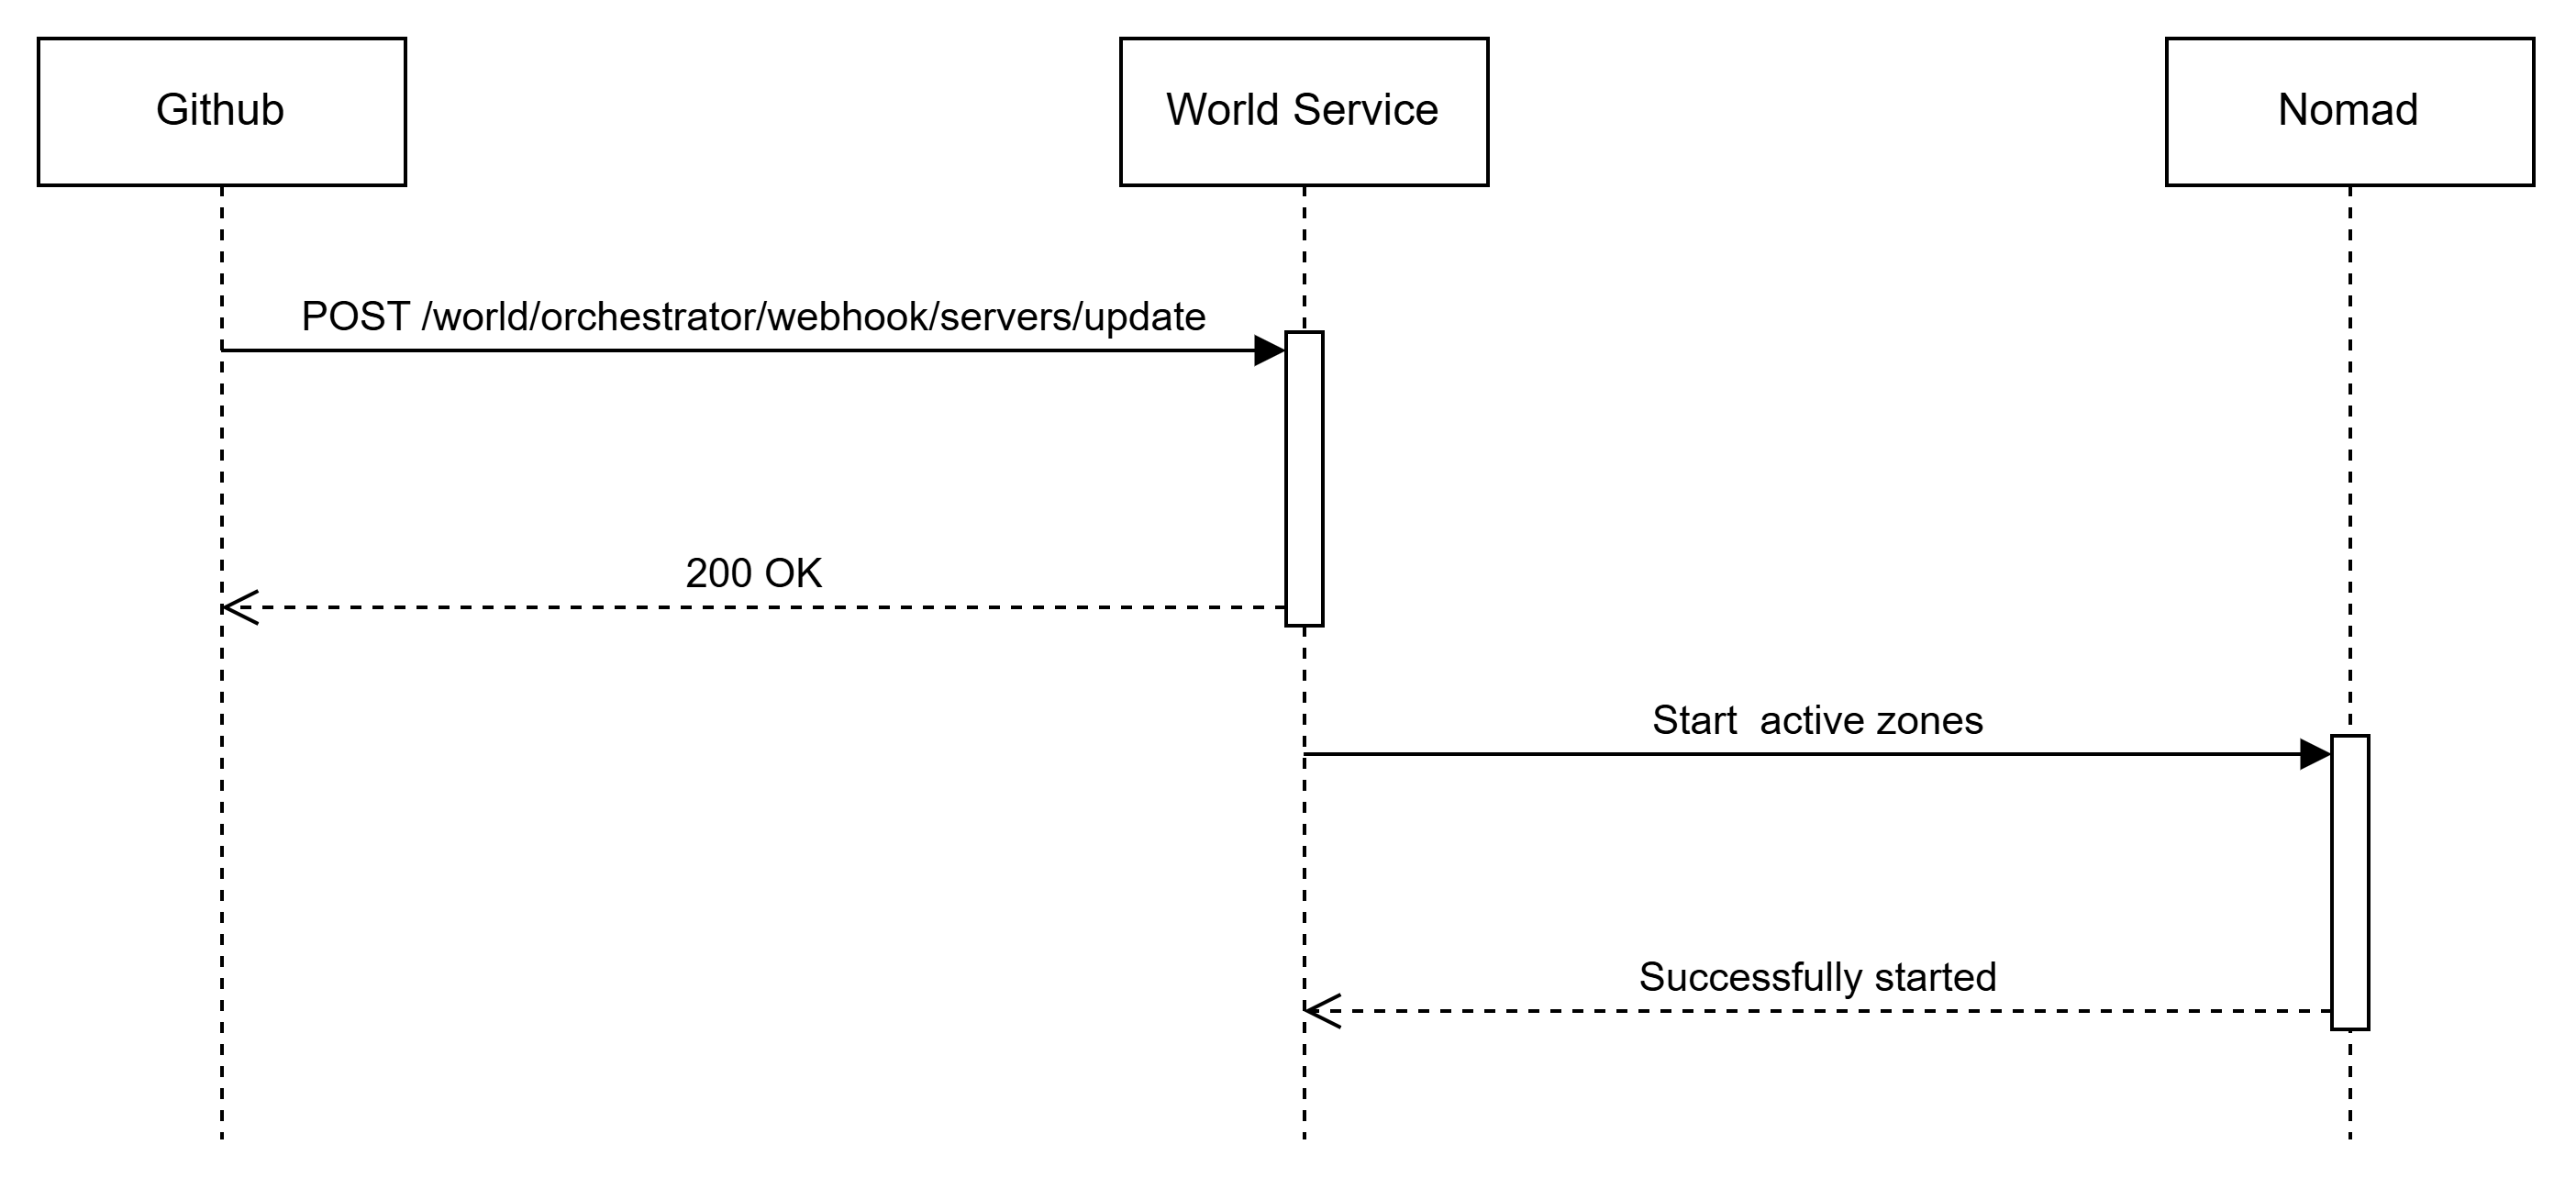
\includegraphics[width=\textwidth]{img/08-implemented-solution/core-service/world-service-case-2.png}
    \caption{Diagrama de secuencia de la actualización de los servidores}
    \label{fig:world-service-case-2}
\end{figure}

Los propios servidores de juego reportan periódicamente su estado al \textit{core service}. Cada 2 minutos
envían el recuento de jugadores activos y el tiempo promedio de sesión mediante
\texttt{POST /world/orchestrator/\{id\}/zones/\{zone\_id\}/players}, y notifican cambios en su estado de
conexión mediante \texttt{POST /world/orchestrator/\{id\}/zones/\{zone\_id\}/status}.
\vspace{0.25cm}

Finalmente, el \textit{endpoint} \texttt{POST /world/orchestrator/webhook/servers/update} permite actualizar todos los
servidores en ejecución ante un nuevo despliegue, por el cambio en una imagen, autenticando la petición mediante un token 
OIDC de GitHub para restringir su uso a los flujos de integración continua.
\vspace{0.25cm}

\underline{\textbf{Endpoints}}

\renewcommand{\arraystretch}{1.4}
\begin{longtable}{|p{2cm}|p{7cm}|p{5.5cm}|}
\hline
\textbf{Verbo HTTP} & \textbf{Path} & \textbf{Descripción} \\
\hline
\endfirsthead

\hline
\textbf{Verbo HTTP} & \textbf{Path} & \textbf{Descripción} \\
\hline
\endhead

\endfoot

\multicolumn{3}{|l|}{\textit{Worlds}} \\
\hline
\texttt{GET}    & \texttt{/world}                                & Retorna la lista paginada de worlds. Soporta filtros por \texttt{user\_id} y texto. \\
\hline
\texttt{POST}   & \texttt{/world}                                & Crea un nuevo world en el registro. \\
\hline
\texttt{GET}    & \texttt{/world/\{id\}}                         & Retorna el detalle completo de un world por su ID. \\
\hline
\texttt{PUT}    & \texttt{/world/\{id\}}                         & Actualiza los datos y descripción de un world. Requiere ownership. \\
\hline
\texttt{DELETE} & \texttt{/world/\{id\}}                         & Elimina un world permanentemente. Requiere ownership. \\
\hline
\texttt{PUT}    & \texttt{/world/\{id\}/createable-data}         & Actualiza el campo \texttt{createable\_data} de un world. Requiere ownership. \\
\hline
\texttt{DELETE} & \texttt{/world/reset-database}                 & Purga todas las tablas. Solo uso en desarrollo. \\
\hline
\multicolumn{3}{|l|}{\textit{Zones}} \\
\hline
\texttt{GET}    & \texttt{/world/\{id\}/zones}                   & Retorna todos los IDs de zonas disponibles para un world. \\
\hline
\texttt{GET}    & \texttt{/world/\{id\}/zones/\{zone\_id\}}      & Retorna los datos de una zona específica de un world. \\
\hline
\texttt{PUT}    & \texttt{/world/\{id\}/zones/\{zone\_id\}}      & Publica o actualiza una zona de un world. Requiere ownership. \\
\hline
\texttt{GET}    & \texttt{/world/\{id\}/zones/\{zone\_id\}/} \newline \texttt{activate}   & Inicia la orquestación de servidores para una zona y consume un slot de suscripción. \\
\hline
\texttt{GET}    & \texttt{/world/\{id\}/zones/\{zone\_id\}/} \newline \texttt{deactivate} & Detiene la orquestación de una zona activa y libera un slot de suscripción. \\
\hline
\texttt{GET}    & \texttt{/world/internal/users/\{user\_id\}/} \newline \texttt{stop-jobs} & Detiene todas las zonas y jobs activos de un usuario. Uso interno entre servicios. \\
\hline
\multicolumn{3}{|l|}{\textit{Orchestrator}} \\
\hline
\texttt{GET}    & \texttt{/world/orchestrator/\{id\}/} \newline \texttt{zones/\{zone\_id\}/start-job} & Inicia un contenedor de servidor de juego en el orquestador para un world y zona. Solo administradores. \\
\hline
\texttt{GET}    & \texttt{/world/orchestrator/\{id\}/} \newline \texttt{zones/\{zone\_id\}/stop-job}  & Detiene el contenedor del orquestador vinculado a un world y zona. Solo administradores. \\
\hline
\texttt{GET}    & \texttt{/world/orchestrator/\{id\}/} \newline \texttt{zones/\{zone\_id\}/address}   & Retorna la IP y puerto del servidor en ejecución para un world y zona. \\
\hline
\texttt{GET}    & \texttt{/world/orchestrator/\{id\}/} \newline \texttt{zones/\{zone\_id\}/status}    & Actualiza el estado online de una zona específica. \\
\hline
\texttt{POST}   & \texttt{/world/orchestrator/\{id\}/} \newline \texttt{zones/\{zone\_id\}/players}   & Los servidores reportan jugadores activos y tiempo promedio cada 2 minutos. \\
\hline
\texttt{GET}    & \texttt{/world/orchestrator/\{id\}/players}    & Retorna los conteos de jugadores por zona para un world. \\
\hline
\texttt{GET}    & \texttt{/world/orchestrator/players}           & Retorna los conteos de jugadores de todos los worlds. \\
\hline
\texttt{POST}   & \texttt{/world/orchestrator/webhook/} \newline \texttt{servers/update} & Webhook para actualizar los servidores en ejecución. Requiere token OIDC de GitHub. \\
\hline
\caption{\textit{Endpoints} del \textit{world service}}
\label{tab:world-endpoints}
\end{longtable}
